\documentclass[tikz]{standalone}
\usepackage{pgfplots}
\pgfplotsset{compat=1.15}
\usepackage{mathrsfs}
\usetikzlibrary{arrows,calc}
\usepackage{tkz-euclide}
\pagestyle{empty}

\definecolor{AngleClr}{rgb}{0,0.39215686274509803,0}
\definecolor{ShapeClr}{rgb}{0.6,0.2,0}

\begin{document}

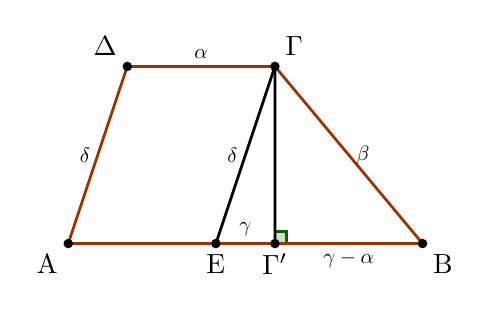
\begin{tikzpicture}[scale=.75]
\tkzSetUpLine[line width=1pt,color=black]
\tkzSetUpPoint[fill=black]

\tkzDefPoints{0/0/A,6/0/B,1/3/D,3.5/3/C}

\tkzDefMidPoint(A,D) \tkzGetPoint{M1}
\tkzDefLine[parallel=through C](D,A) \tkzGetPoint{x}

\tkzInterLL(C,x)(A,B)\tkzGetPoint{E}

\tkzDefPointBy[projection=onto A--B](C) \tkzGetPoint{C'}

\tkzFillPolygon[fill=white](A,B,C,D)

\tkzMarkRightAngle[line width=1pt, size=.2,color=AngleClr,fill=AngleClr,fill opacity=0.2](C,C',B)

\tkzDrawSegments(C,E C,C')
% \tkzDrawSegments[dashed, line width=0.5,dash pattern=on 1pt off 1.75pt](M1,E C,E)

\tkzDrawPolygon[color=ShapeClr](A,B,C,D)
\tkzDrawPoints[size=3](A,B,C,D,E,C')
\tkzLabelPoint[below left](A){$\rm A$}
\tkzLabelPoint[below right](B){$\rm B$}
\tkzLabelPoint[above right](C){$\rm \Gamma$}
\tkzLabelPoint[above left](D){$\rm \Delta$}
\tkzLabelPoint[below](E){$\rm E$}
\tkzLabelPoint[below](C'){$\rm \Gamma'$}

\tkzLabelSegment[below,scale=0.75](C',B){$\gamma - \alpha$}
\tkzLabelSegments[left,scale=0.75](A,D C,E){$\delta$}
\tkzLabelSegment[right,scale=0.75](B,C){$\beta$}
\tkzLabelSegment[above,scale=0.75](C,D){$\alpha$}
\tkzLabelSegment[above,scale=0.75](A,B){$\gamma$}


\end{tikzpicture}
\end{document}
